\ifdefined\inMainDoc\else
\documentclass[12pt,a4paper]{article}
% ================================================================
%  PRÉAMBULE COMMUN - ANNALES CORRIGÉES
%  Université de Kara - FaST - Licence Fondamentale MPC
%  Design optimisé impression noir et blanc
% ================================================================

% -- ENCODAGE & LANGUE --
\usepackage[utf8]{inputenc}
\usepackage[T1]{fontenc}
\usepackage[french]{babel}
\usepackage{lmodern}
\usepackage{microtype}

% -- MISE EN PAGE --
\usepackage[a4paper, top=2.8cm, bottom=2.5cm, left=2.5cm, right=2.5cm, headheight=14pt]{geometry}
\usepackage{setspace}
\setstretch{1.2}
\usepackage{parskip}
\setlength{\parindent}{1.2em}
\setlength{\parskip}{4pt}

% -- MATHS --
\usepackage{amsmath, amssymb, mathtools, amsthm}
\usepackage{mathrsfs}
\usepackage{dsfont}
\usepackage{bm}
\usepackage{cancel}
\usepackage{textcomp}
% Définition de \oiint (intégrale de surface fermée) sans package supplémentaire
\newcommand{\oiint}{\mathop{\iint\!\!\!\!\!\!\!\bigcirc}\limits}

% -- PHYSIQUE & CHIMIE --
\usepackage{physics}
\usepackage{siunitx}
% Lorsque physics est chargé, siunitx omet \qty. On le restaure ici :
\AtBeginDocument{\RenewCommandCopy\qty\SI}
\sisetup{locale = FR, detect-all, output-decimal-marker={,}}
% Commande de substitution pour les unités posant problème avec pdflatex
% (ohm, degreeCelsius, micro, angstrom, percent utilisent des caractères non-ASCII)
\newcommand{\qtyohm}[1]{\ensuremath{\num{#1}\,\Omega}}
\newcommand{\qtydegc}[1]{\ensuremath{\num{#1}\,{}^\circ\text{C}}}
\newcommand{\qtyangstrom}[1]{\ensuremath{\num{#1}\,\text{\AA}}}
\newcommand{\qtypercent}[1]{\ensuremath{\num{#1}\,\%}}
\newcommand{\qtyum}[1]{\ensuremath{\num{#1}\,\mu\text{m}}}
\usepackage[version=4]{mhchem}

% -- GRAPHISMES --
\usepackage{graphicx}
\usepackage{float}
\usepackage{caption}
\usepackage{subcaption}
\usepackage{wrapfig}
\usepackage{tikz}
\usetikzlibrary{calc, arrows.meta, patterns, shapes.geometric}
\usepackage{pgfplots}
\pgfplotsset{compat=1.18}

% -- TABLEAUX --
\usepackage{booktabs}
\usepackage{array}
\usepackage{tabularx}
\usepackage{multirow}

% -- LISTES --
\usepackage{enumitem}
\setlist[enumerate]{topsep=3pt, itemsep=2pt, parsep=0pt}
\setlist[itemize]{topsep=3pt, itemsep=2pt, parsep=0pt, label={.}}

% -- BOÎTES (noir et blanc) --
\usepackage{mdframed}
\usepackage{tcolorbox}
\tcbuselibrary{skins, breakable, theorems}

% Boîte EXERCICE : encadré avec filet épais, fond blanc
\newmdenv[
  linewidth=1.2pt,
  linecolor=black,
  roundcorner=3pt,
  skipabove=10pt,
  skipbelow=6pt,
  innertopmargin=8pt,
  innerbottommargin=8pt,
  innerleftmargin=10pt,
  innerrightmargin=10pt,
  backgroundcolor=white,
  frametitle={\bfseries\small Exercice},
  frametitlealignment=\raggedright,
  frametitleaboveskip=4pt,
  frametitlebelowskip=4pt,
]{boiteexercice}

% Boîte CORRIGÉ : fond gris très clair + filet fin
\newmdenv[
  linewidth=0.6pt,
  linecolor=black,
  leftline=true,
  rightline=false,
  topline=false,
  bottomline=false,
  linecolor=black,
  innerleftmargin=12pt,
  innerrightmargin=8pt,
  innertopmargin=6pt,
  innerbottommargin=6pt,
  backgroundcolor=gray!8,
  skipabove=4pt,
  skipbelow=8pt,
]{boitecorrige}

% Boîte RÉSUMÉ DE COURS : double encadré
\newmdenv[
  linewidth=0.8pt,
  linecolor=black,
  roundcorner=2pt,
  backgroundcolor=gray!12,
  innertopmargin=10pt,
  innerbottommargin=10pt,
  innerleftmargin=12pt,
  innerrightmargin=12pt,
  skipabove=12pt,
  skipbelow=8pt,
]{boiteresume}

% Boîte ATTENTION/REMARQUE : barre gauche épaisse
\newmdenv[
  leftline=true,
  rightline=false,
  topline=false,
  bottomline=false,
  linewidth=3pt,
  linecolor=black,
  backgroundcolor=gray!5,
  innerleftmargin=12pt,
  innerrightmargin=8pt,
  innertopmargin=5pt,
  innerbottommargin=5pt,
  skipabove=6pt,
  skipbelow=6pt,
]{boiteremarque}

% -- DIFFICULTÉ DES EXERCICES --
\newcommand{\facile}{$\star$}
\newcommand{\moyen}{$\star\!\star$}
\newcommand{\difficile}{$\star\!\star\!\star$}
\newcommand{\niveau}[1]{\hfill\textbf{#1}\hspace{2pt}}

% -- EN-TÊTES ET PIEDS DE PAGE --
\usepackage{fancyhdr}
\pagestyle{fancy}
\fancyhf{}
\renewcommand{\headrulewidth}{0.5pt}
\renewcommand{\footrulewidth}{0.3pt}

% -- HYPERLIENS --
\usepackage[hidelinks]{hyperref}
\hypersetup{
    colorlinks=false,
    pdftitle={Annale Corrigée - Licence MPC - Université de Kara}
}

% -- TITRES --
\usepackage{titlesec}
\titleformat{\section}{\Large\bfseries}{\thesection.}{0.8em}{}[\vspace{2pt}\hrule\vspace{4pt}]
\titleformat{\subsection}{\large\bfseries}{\thesubsection.}{0.7em}{}
\titleformat{\subsubsection}{\normalsize\bfseries}{\thesubsubsection.}{0.6em}{}

% -- THÉORÈMES --
\theoremstyle{definition}
\newtheorem{defn}{Définition}[section]
\newtheorem{prop}{Propriété}[section]
\newtheorem{thm}{Théorème}[section]
\newtheorem{corol}{Corollaire}[section]
\newtheorem{exemple}{Exemple}[section]

% -- COMMANDES MATHÉMATIQUES UTILES --
\newcommand{\vect}[1]{\overrightarrow{#1}}
\newcommand{\R}{\mathbb{R}}
\newcommand{\N}{\mathbb{N}}
\newcommand{\Z}{\mathbb{Z}}
\newcommand{\C}{\mathbb{C}}
\renewcommand{\d}{\mathrm{d}}
\newcommand{\deriv}[2]{\dfrac{\d #1}{\d #2}}
\newcommand{\dpart}[2]{\dfrac{\partial #1}{\partial #2}}
\newcommand{\rot}{\overrightarrow{\mathrm{rot}}\,}
\renewcommand{\div}{\mathrm{div}\,}
\renewcommand{\grad}{\overrightarrow{\mathrm{grad}}\,}
\newcommand{\e}{\mathrm{e}}
\newcommand{\ii}{\mathrm{i}}
\renewcommand{\Tr}{\mathrm{Tr}}

% Numérotation des équations par section
\numberwithin{equation}{section}

% -- RÉSULTATS ENCADRÉS --
\newcommand{\res}[1]{\[\boxed{#1}\]}

% -- REMARQUE INLINE --
\newcommand{\rmq}[1]{\begin{boiteremarque}\textbf{Remarque.} #1\end{boiteremarque}}

% -- MISE EN VALEUR DU RÉSULTAT FINAL --
\newcommand{\reponse}[1]{%
  \begin{center}
    \fbox{\begin{minipage}{0.92\textwidth}\centering #1\end{minipage}}
  \end{center}%
}


\lhead{\small\textit{Électromagnétisme - Licence 2}}
\rhead{\small\textit{FaST, Université de Kara}}
\cfoot{\thepage}

\begin{document}
\fi

\begin{center}
  {\LARGE\bfseries ÉLECTROMAGNÉTISME}\\[0.3cm]
  {\normalsize Licence 2 - Mathématiques, Physique et Chimie}\\[0.1cm]
  \rule{0.7\textwidth}{0.8pt}
\end{center}

\vspace{0.3cm}

% ================================================================
\section*{Résumé du cours}
% ================================================================

\begin{boiteresume}

\textbf{1. Équations de Maxwell (dans le vide).}
\[
\div\vec{E} = \frac{\rho}{\varepsilon_0} \qquad \div\vec{B} = 0
\]
\[
\rot\vec{E} = -\dpart{\vec{B}}{t} \qquad \rot\vec{B} = \mu_0\left(\vec{j} + \varepsilon_0\dpart{\vec{E}}{t}\right)
\]
avec $c = 1/\sqrt{\varepsilon_0\mu_0} \approx \qty{3e8}{m.s^{-1}}$.

\textbf{2. Ondes électromagnétiques planes.} Une onde plane progressive harmonique (OPPH) se propageant selon $Ox$ s'écrit $\vec{E}(x,t) = E_0\,\hat{e}_\perp\,\cos(kx - \omega t)$, avec $k = \omega/c$. Les champs $\vec{E}$ et $\vec{B}$ sont perpendiculaires entre eux et à la direction de propagation. La relation de Poynting donne l'intensité moyenne :
\[
\langle S \rangle = \frac{E_{0}^2}{2\mu_0 c} = \frac{P}{4\pi r^2}
\]
pour une source isotropique de puissance $P$ à distance $r$.

\textbf{3. Induction électromagnétique.} La force électromotrice (f.é.m.) induite dans un circuit soumis à un flux magnétique variable est (loi de Faraday) :
\[
e = -\deriv{\Phi}{t}
\]
La loi de Lenz précise que la f.é.m. induite crée un courant qui s'oppose à la cause qui l'engendre.

\textbf{4. Vecteur de Poynting et énergie.} $\vec{\Pi} = \frac{1}{\mu_0}\vec{E}\wedge\vec{B}$ représente la densité de flux d'énergie électromagnétique. La densité volumique d'énergie est $u_{em} = \frac{1}{2}\varepsilon_0 E^2 + \frac{1}{2\mu_0}B^2$.

\end{boiteresume}

\newpage

% ================================================================
\section{Ondes électromagnétiques}
% ================================================================

\subsection*{Exercice 1 - Portée d'un talkie-walkie \niveau{\moyen}}

\begin{boiteexercice}
Un talkie-walkie émet à la fréquence $f = \qty{446}{MHz}$ avec une puissance $P = \qty{0.5}{W}$. Il peut détecter un champ électrique de valeur efficace $E_{rms} = \qty{1.5}{mV.m^{-1}}$.

Calculer la portée maximale de cet appareil.
\end{boiteexercice}

\begin{boitecorrige}
La puissance rayonnée par une antenne isotropique se répartit uniformément sur une sphère de rayon $r$. La densité de flux (intensité du vecteur de Poynting) à distance $r$ est :
\[
\langle\Pi\rangle = \frac{P}{4\pi r^2}
\]
Or, la relation entre le champ électrique efficace et le vecteur de Poynting dans le vide est :
\[
\langle\Pi\rangle = \frac{E_{rms}^2}{\mu_0 c}
\]
En égalant ces deux expressions :
\[
\frac{E_{rms}^2}{\mu_0 c} = \frac{P}{4\pi r^2} \quad \Rightarrow \quad r = \frac{1}{E_{rms}}\sqrt{\frac{\mu_0 c P}{4\pi}}
\]

Application numérique :
\[
r = \frac{1}{1{,}5\times10^{-3}}\sqrt{\frac{4\pi\times10^{-7}\times3\times10^8\times0{,}5}{4\pi}}
= \frac{1}{1{,}5\times10^{-3}}\sqrt{\frac{10^{-7}\times3\times10^8\times0{,}5}{1}}
\]
\[
r = \frac{1}{1{,}5\times10^{-3}}\sqrt{1{,}5\times10^{-2}\times 3\times10^8\times \frac{1}{4\pi}}
\]

Calcul numérique détaillé : $\mu_0 c = 4\pi\times10^{-7}\times3\times10^8 = 120\pi \approx \qtyohm{377}$.
\[
r = \frac{1}{E_{rms}}\sqrt{\frac{\mu_0 c\, P}{4\pi}}
  = \frac{1}{1{,}5\times10^{-3}}\sqrt{\frac{377\times0{,}5}{4\pi}}
\]
\[
  \approx \frac{1}{1{,}5\times10^{-3}}\sqrt{15}
  \approx \frac{3{,}87}{1{,}5\times10^{-3}} \approx \qty{2.58}{km}
\]

La portée maximale est d'environ $\qty{2.6}{km}$.

\begin{boiteremarque}
La formule correcte utilise $E_{rms}^2 = \mu_0 c \langle\Pi\rangle$, et non $\varepsilon_0 c^2$ au dénominateur. Dans le vide, $\mu_0 c = \sqrt{\mu_0/\varepsilon_0} \approx \qtyohm{377}$ (impédance du vide).
\end{boiteremarque}
\end{boitecorrige}

\subsection*{Exercice 2 - Expressions des ondes planes \niveau{\moyen}}

\begin{boiteexercice}
Donner les expressions réelles $\vec{E}(\vec{r},t)$ des ondes planes progressives harmoniques suivantes dans le vide :
\begin{enumerate}
  \item Une onde d'amplitude $E_0$ se propageant suivant $Ox$ et polarisée linéairement à $\pi/3$ de $Oy$.
  \item Une onde d'amplitude $E_0$ polarisée linéairement suivant $Oy$ et se propageant parallèlement au plan $zOx$ à $\pi/4$ de $Oz$.
\end{enumerate}
\end{boiteexercice}

\begin{boitecorrige}
\textbf{1.} Le vecteur d'onde est $\vec{k} = k\,\hat{i}$ avec $k = \omega/c$. La polarisation à $\pi/3$ de $Oy$ dans le plan $yOz$ donne :
\[
\boxed{\vec{E}(x,t) = E_0\left(\cos\frac{\pi}{3}\,\hat{j} + \sin\frac{\pi}{3}\,\hat{k}\right)\cos(kx-\omega t) = E_0\left(\frac{1}{2}\,\hat{j} + \frac{\sqrt{3}}{2}\,\hat{k}\right)\cos(kx-\omega t)}
\]

\textbf{2.} L'onde se propage dans le plan $zOx$ à $\pi/4$ de $Oz$, donc $\vec{k} = \frac{k}{\sqrt{2}}(\hat{i}+\hat{k})$. Polarisée selon $Oy$ :
\[
\boxed{\vec{E}(x,z,t) = E_0\,\hat{j}\,\cos\!\left(\frac{k}{\sqrt{2}}(x+z) - \omega t\right)}
\]
\end{boitecorrige}

\subsection*{Exercice 3 - Équations de Maxwell et induction \niveau{\difficile}}

\begin{boiteexercice}
\begin{enumerate}
  \item Montrer que $e = -\d\Phi/\d t$ est équivalent à $\rot\vec{E} = -\partial\vec{B}/\partial t$.
  \item Montrer que l'équation de continuité $\div\vec{j} + \partial\rho/\partial t = 0$ est contenue dans les équations de Maxwell.
  \item Montrer que $\rot\vec{B} = \mu_0\vec{j}$ est la forme locale du théorème d'Ampère en régime permanent.
\end{enumerate}
\end{boiteexercice}

\begin{boitecorrige}
\textbf{1.} On intègre $\rot\vec{E} = -\partial\vec{B}/\partial t$ sur une surface $S$ s'appuyant sur le contour $C$ :
\[
\iint_S \rot\vec{E}\cdot\d\vec{S} = -\iint_S \frac{\partial\vec{B}}{\partial t}\cdot\d\vec{S}
\]
Le théorème de Stokes transforme le membre gauche :
\[
\oint_C \vec{E}\cdot\d\vec{l} = -\frac{\partial}{\partial t}\iint_S \vec{B}\cdot\d\vec{S} = -\frac{\d\Phi}{\d t}
\]
Or, $e = \oint_C \vec{E}\cdot\d\vec{l}$, ce qui établit bien $e = -\d\Phi/\d t$.

Physiquement, Maxwell-Faraday traduit qu'un champ magnétique variable engendre un champ électrique.

\textbf{2.} Prenons la divergence de l'équation de Maxwell-Ampère :
\[
\div(\rot\vec{B}) = 0 \Rightarrow \mu_0\div\!\left(\vec{j}+\varepsilon_0\frac{\partial\vec{E}}{\partial t}\right) = 0
\]
\[
\div\vec{j} + \varepsilon_0\frac{\partial}{\partial t}(\div\vec{E}) = 0 \Rightarrow \div\vec{j} + \varepsilon_0\frac{\partial}{\partial t}\!\left(\frac{\rho}{\varepsilon_0}\right) = 0
\]
\[
\boxed{\div\vec{j} + \frac{\partial\rho}{\partial t} = 0}
\]

\textbf{3.} En régime permanent, $\partial\vec{E}/\partial t = 0$, donc Maxwell-Ampère se réduit à $\rot\vec{B} = \mu_0\vec{j}$. En intégrant sur une surface $S$ et en appliquant Stokes :
\[
\oint_C\vec{B}\cdot\d\vec{l} = \mu_0\iint_S\vec{j}\cdot\d\vec{S} = \mu_0\,I
\]
C'est bien le théorème d'Ampère en régime permanent.
\end{boitecorrige}

\subsection*{Exercice 4 - Induction : barre sur rails verticaux \niveau{\moyen}}

\begin{boiteexercice}
Une barre homogène MN de masse $m$ se déplace sur deux rails verticaux distants de $\ell$, reliés par une résistance $R$ en leurs parties supérieures. Le tout est plongé dans un champ $\vec{B}_0$ uniforme et perpendiculaire au plan des rails. La barre est lâchée sans vitesse initiale à $t=0$.

\begin{enumerate}
  \item Exprimer la variation de flux $\d\Phi$ induite par le mouvement si la vitesse à l'instant $t$ est $v$.
  \item Calculer la f.é.m. $e$ et le courant $i$.
  \item Exprimer la force électromagnétique $F$ sur la barre.
  \item Établir la loi $v(t)$, en négligeant les frottements.
\end{enumerate}
\end{boiteexercice}

\begin{boitecorrige}
\textbf{1.} En prenant le sens positif vers le bas, si la barre descend d'une distance $\d x = v\,\d t$ :
\[
\d\Phi = B_0\,\ell\,v\,\d t
\]

\textbf{2.} La f.é.m. d'induction (loi de Faraday) :
\[
e = -\deriv{\Phi}{t} = -B_0\,\ell\,v(t)
\]
Le courant dans la résistance $R$ :
\[
i = \frac{|e|}{R} = \frac{B_0\,\ell\,v(t)}{R}
\]
La loi de Lenz confirme que ce courant crée une force qui s'oppose au mouvement (frein électromagnétique).

\textbf{3.} La force de Laplace sur la barre (de longueur $\ell$ parcourue par $i$, dans le champ $B_0$) est verticale, dirigée vers le haut (frein) :
\[
F = i\,\ell\,B_0 = \frac{B_0^2\,\ell^2\,v}{R}
\]

\textbf{4.} Le principe fondamental de la dynamique sur la barre (poids $mg$ vers le bas, force de Laplace $F$ vers le haut) :
\[
m\deriv{v}{t} = mg - \frac{B_0^2\,\ell^2}{R}\,v
\]
C'est une équation différentielle du premier ordre avec second membre constant. En posant $v_\infty = mgR/(B_0^2\ell^2)$ et $\tau = mR/(B_0^2\ell^2)$ :
\[
\boxed{v(t) = v_\infty\left(1 - \e^{-t/\tau}\right) = \frac{mgR}{B_0^2\ell^2}\left(1 - \e^{-\frac{B_0^2\ell^2}{mR}t}\right)}
\]
La vitesse tend asymptotiquement vers $v_\infty$ (vitesse limite).
\end{boitecorrige}

% ================================================================
\section{Ondes dans les milieux}
% ================================================================

\subsection*{Exercice 5 - Onde dans un guide \niveau{\difficile}}

\begin{boiteexercice}
On considère le champ électrique $\vec{E} = E_0\cos(\alpha z)\sin(\omega t - kx)\,\hat{u}_y$ dans le vide.
\begin{enumerate}
  \item Cette onde est-elle plane ? Progressive ? Harmonique ?
  \item Calculer le champ magnétique.
  \item Y a-t-il dispersion ?
\end{enumerate}
\end{boiteexercice}

\begin{boitecorrige}
\textbf{1.} L'onde n'est pas \textbf{plane} (la dépendance en $z$ via $\cos(\alpha z)$ ne correspond pas à une propagation dans une seule direction). Elle est en revanche \textbf{progressive} (dépendance en $kx - \omega t$) et \textbf{harmonique} (sinusoïdale en temps et en espace). Ce type d'onde se rencontre typiquement dans les guides d'ondes.

\textbf{2.} En utilisant Maxwell-Faraday $\rot\vec{E} = -\partial\vec{B}/\partial t$ et en intégrant :
\[
B_x = \frac{E_0\,\alpha}{\omega}\sin(\alpha z)\cos(\omega t - kx) \qquad B_z = \frac{k\,E_0}{\omega}\cos(\alpha z)\sin(\omega t - kx)
\]

\textbf{3.} En substituant $\vec{E}$ dans l'équation de d'Alembert $\Delta\vec{E} = \frac{1}{c^2}\frac{\partial^2\vec{E}}{\partial t^2}$ :
\[
-(\alpha^2 + k^2)E_0\cos(\alpha z)\sin(\omega t - kx) = -\frac{\omega^2}{c^2}E_0\cos(\alpha z)\sin(\omega t - kx)
\]
\[
\boxed{k^2 = \frac{\omega^2}{c^2} - \alpha^2}
\]
Oui, il y a \textbf{dispersion} : la relation de dispersion n'est pas linéaire. La vitesse de phase est :
\[
v_\varphi = \frac{\omega}{k} = \frac{c}{\sqrt{1 - \frac{\alpha^2 c^2}{\omega^2}}} > c
\]
\end{boitecorrige}

\subsection*{Exercice 6 - Guide d'onde et énergie \niveau{\difficile}}

\newpage
\begin{boiteexercice}
Le demi-espace $z < 0$ est un conducteur parfait. Dans le demi-espace $z > 0$, on a :
\[
\vec{E} = E_0\sin(\alpha z)\cos(\omega t - kx)\,\hat{u}_y
\]
\[
\vec{B} = \frac{\alpha E_0}{\omega}\cos(\alpha z)\sin(\omega t - kx)\,\hat{u}_x + \frac{kE_0}{\omega}\sin(\alpha z)\cos(\omega t - kx)\,\hat{u}_z
\]
avec $\omega > c\alpha$.

\begin{enumerate}
  \item Exprimer la relation de dispersion et la vitesse de phase $v_\varphi$.
  \item Calculer la moyenne spatio-temporelle du vecteur de Poynting et de la densité d'énergie électromagnétique.
  \item En déduire la vitesse de propagation de l'énergie $v_E$.
  \item Déterminer la densité de charge $\sigma$ et le courant surfacique $\vec{j}_s$ à la surface du conducteur.
\end{enumerate}
\end{boiteexercice}

\begin{boitecorrige}
\textbf{1.} En substituant $\vec{E}$ dans l'équation de d'Alembert :
\[
k^2 = \frac{\omega^2}{c^2} - \alpha^2 \qquad \text{et} \qquad v_\varphi = \frac{\omega}{k} = \frac{c}{\sqrt{1-\frac{\alpha^2 c^2}{\omega^2}}} > c
\]
La vitesse de groupe $v_g = \d\omega/\d k$ est obtenue en différentiant la relation de dispersion :
$v_g = c\sqrt{1-\frac{\alpha^2 c^2}{\omega^2}} < c$. On vérifie $v_\varphi\cdot v_g = c^2$.

\textbf{2.} Après calcul des moyennes temporelles :
\[
\langle\vec{\Pi}\rangle = \frac{kE_0^2}{4\mu_0\omega}\,\hat{u}_x \qquad \langle u_{em}\rangle = \frac{\varepsilon_0 E_0^2}{4}
\]

\textbf{3.} Un bilan énergétique $\langle u_{em}\rangle\,v_E = \langle\Pi\rangle$ donne :
\[
v_E = \frac{\langle\Pi\rangle}{\langle u_{em}\rangle} = \frac{kc^2}{\omega} = v_g
\]
La vitesse de propagation de l'énergie est égale à la vitesse de groupe.

\textbf{4.} À la surface $z=0$ : le champ électrique est $\vec{E}(z=0) = 0$ (sin$(0)=0$), donc la densité de charge surfacique est $\sigma = \varepsilon_0 E_n = 0$.

Le champ magnétique à la surface vaut $\vec{B}(z=0) = \frac{\alpha E_0}{\omega}\sin(\omega t - kx)\,\hat{u}_x$. La relation de passage pour un conducteur parfait $\vec{B}_{surface} = \mu_0\vec{j}_s\wedge\hat{n}$ (avec $\hat{n} = \hat{u}_z$) donne :
\[
\vec{j}_s = \frac{\alpha E_0}{\mu_0\omega}\sin(\omega t - kx)\,\hat{u}_y
\]
\end{boitecorrige}

% ================================================================
\section{Examens corrigés}
% ================================================================

\subsection*{Examen - Propagation d'onde, polarisation et réflexion \niveau{\difficile}}

\begin{boiteexercice}
\begin{center}
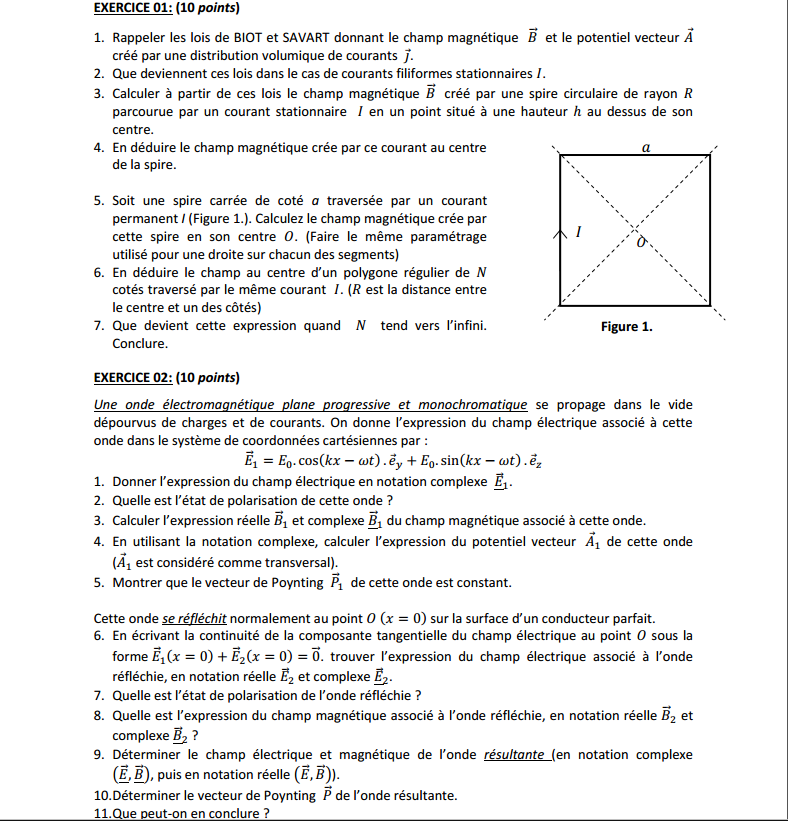
\includegraphics[width=0.9\textwidth]{images/ggg.png}
\end{center}
\end{boiteexercice}

\begin{boitecorrige}
\textbf{Questions 1 à 5 :}
\begin{center}
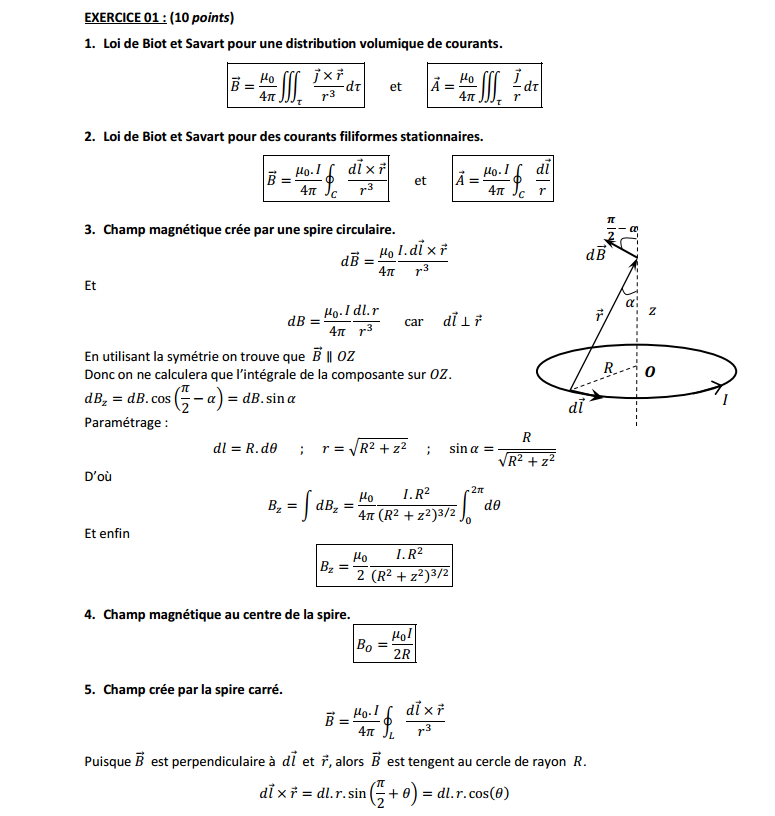
\includegraphics[width=0.92\textwidth]{images/g1.png}
\end{center}
\begin{center}
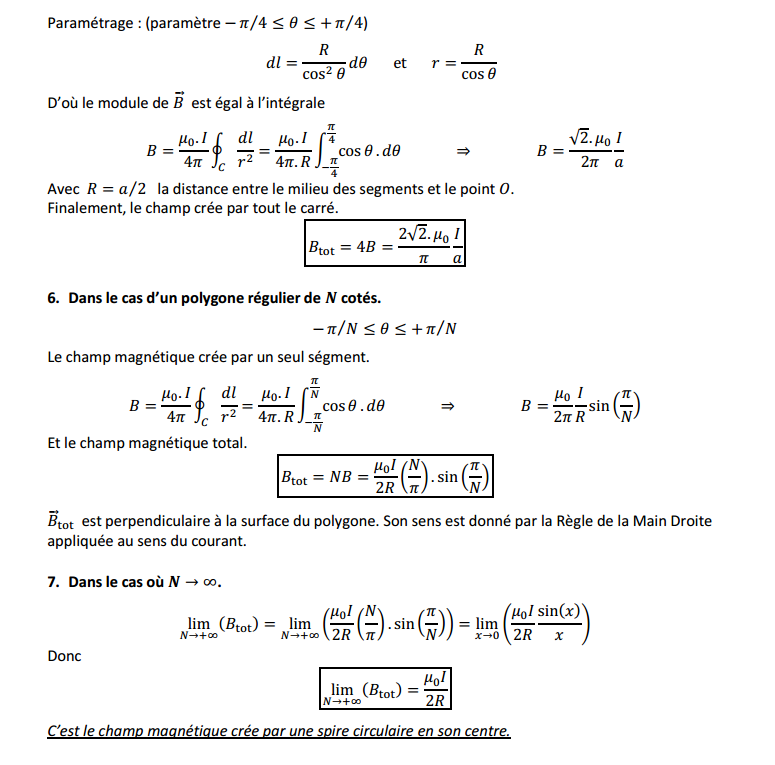
\includegraphics[width=0.92\textwidth]{images/g2.png}
\end{center}
\begin{center}
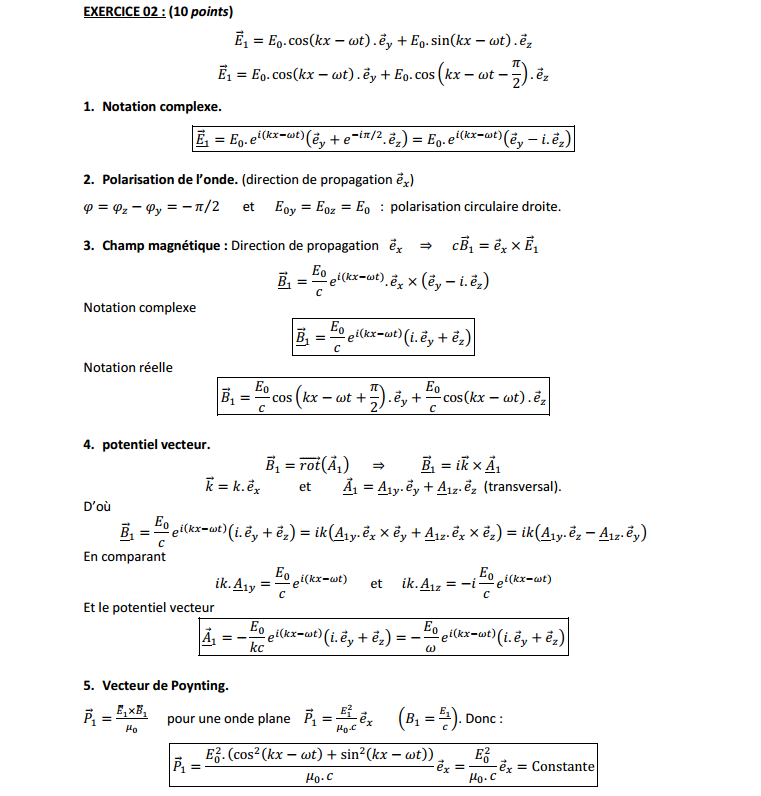
\includegraphics[width=0.92\textwidth]{images/g3.png}
\end{center}

\textbf{Question 6 :} La condition de continuité du champ électrique tangentiel à l'interface impose $\vec{E}_1(x=0) + \vec{E}_2(x=0) = \vec{0}$. L'onde $\vec{E}_2$ est une OPPH se propageant dans la direction des $x$ négatifs. On écrit sa forme générale :
\[
\vec{E}_2 = E_{0y}\cos(kx+\omega t+\varphi_y)\,\hat{e}_y + E_{0z}\cos(kx+\omega t+\varphi_z)\,\hat{e}_z
\]
La condition de continuité en $x=0$ :
\[
-E_0\cos(-\omega t)\,\hat{e}_y - E_0\cos\!\left(-\omega t-\frac{\pi}{2}\right)\hat{e}_z = E_{0y}\cos(\omega t+\varphi_y)\,\hat{e}_y + E_{0z}\cos(\omega t+\varphi_z)\,\hat{e}_z
\]

\begin{center}
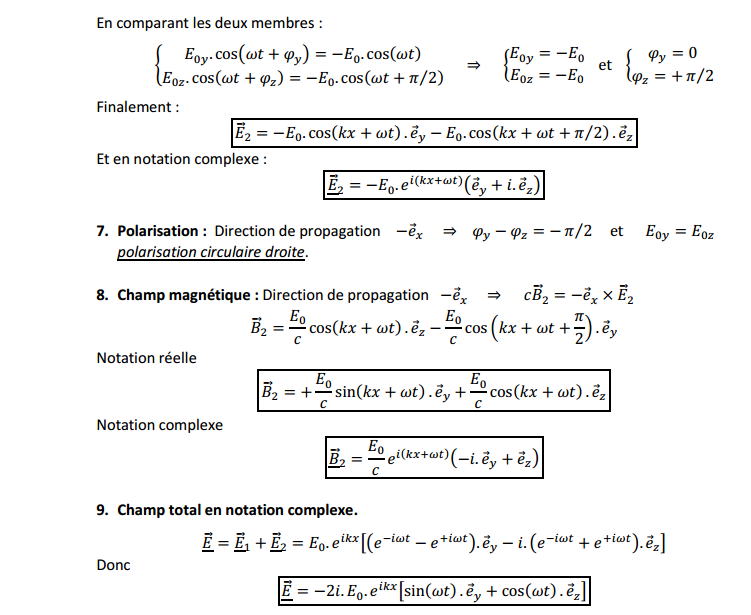
\includegraphics[width=0.9\textwidth]{images/g5.png}
\end{center}
\begin{center}
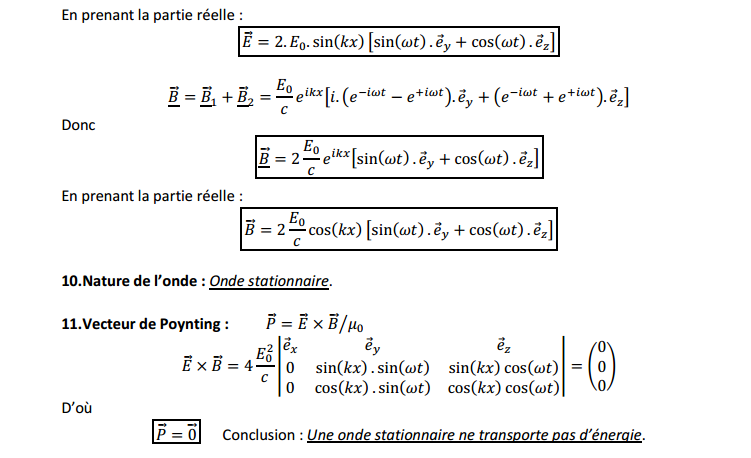
\includegraphics[width=0.9\textwidth]{images/g6.png}
\end{center}
\begin{center}
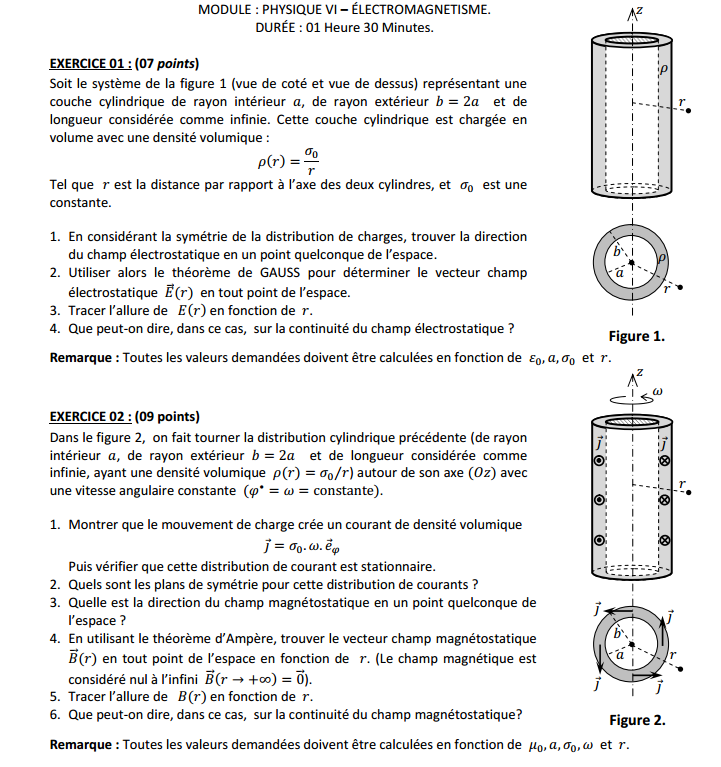
\includegraphics[width=0.9\textwidth]{images/g8.png}
\end{center}
\begin{center}
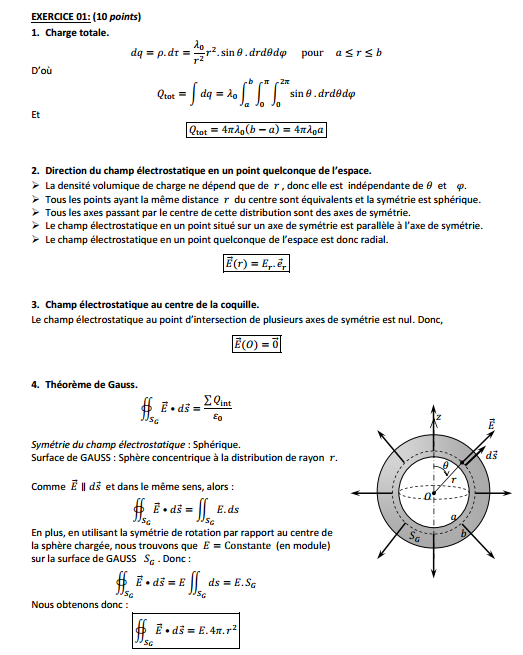
\includegraphics[width=0.9\textwidth]{images/g7.png}
\end{center}
\begin{center}
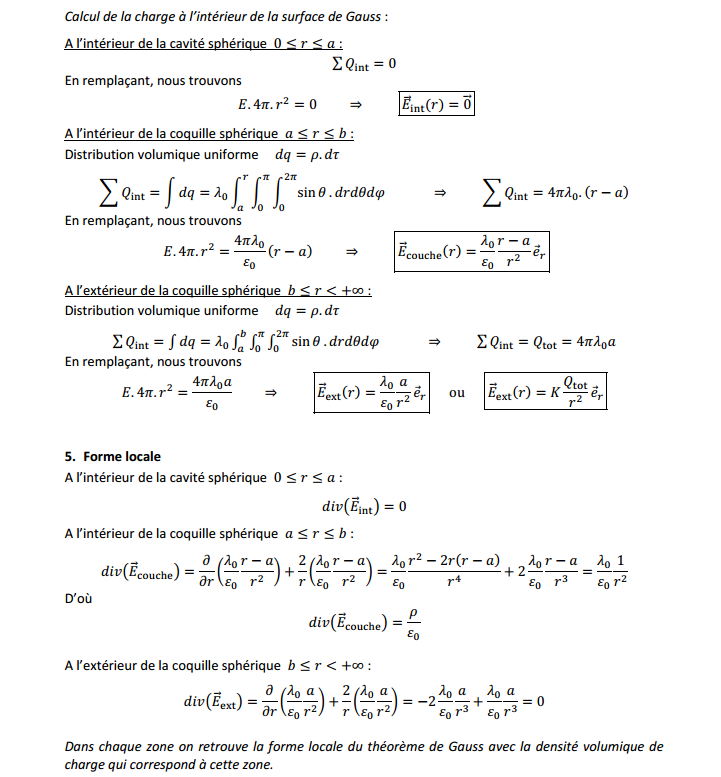
\includegraphics[width=0.9\textwidth]{images/g9.png}
\end{center}
\begin{center}
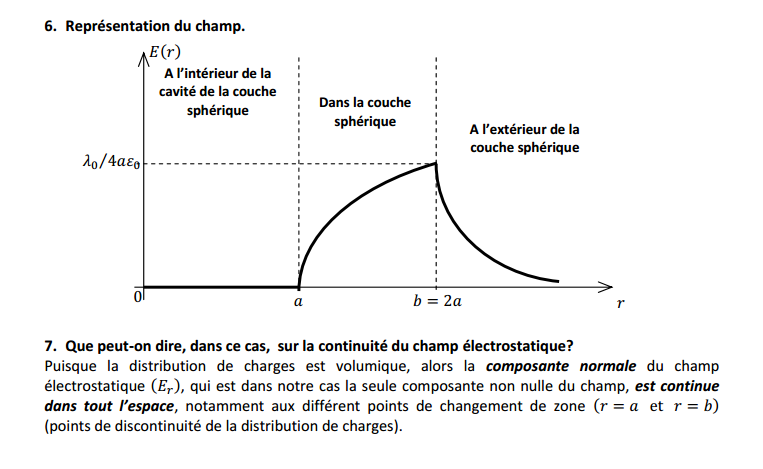
\includegraphics[width=0.9\textwidth]{images/g10.png}
\end{center}
\begin{center}
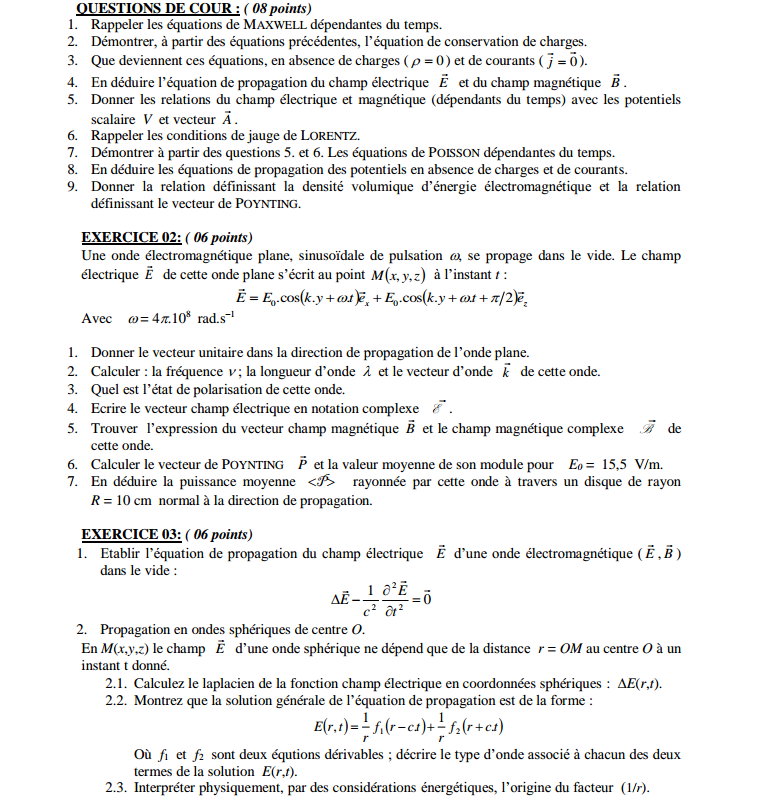
\includegraphics[width=0.9\textwidth]{images/g11.png}
\end{center}
\begin{center}
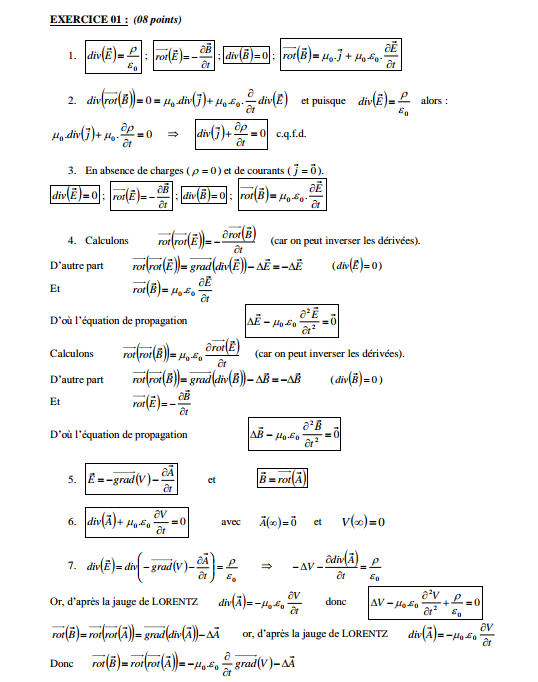
\includegraphics[width=0.9\textwidth]{images/g12.png}
\end{center}
\begin{center}
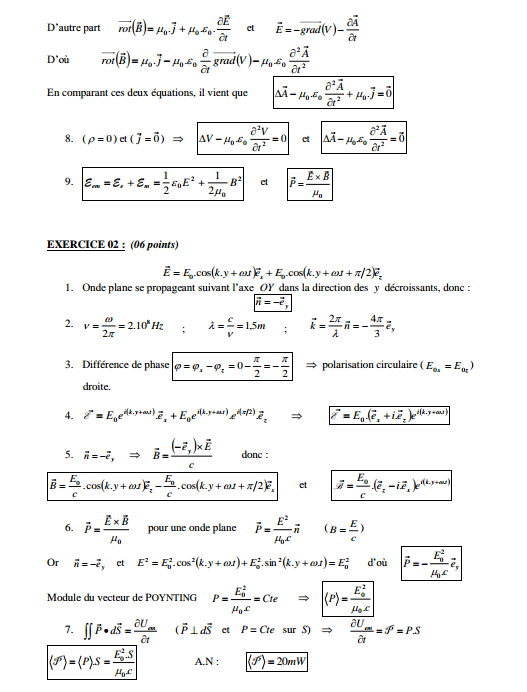
\includegraphics[width=0.9\textwidth]{images/g16.png}
\end{center}
\begin{center}
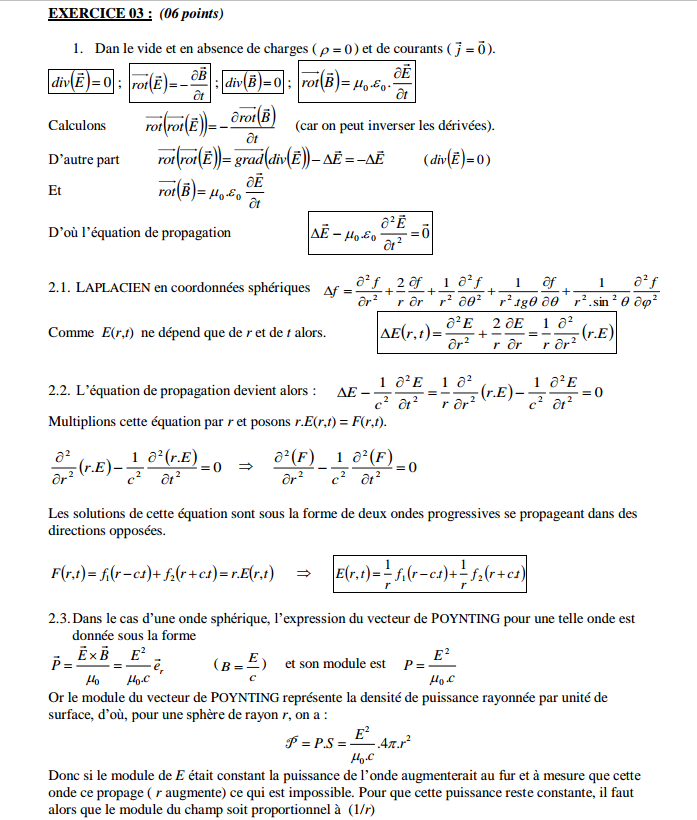
\includegraphics[width=0.9\textwidth]{images/g17.png}
\end{center}

Pour une source isotropique, la conservation de la puissance donne $\mathcal{P} = \langle\Pi\rangle\cdot 4\pi r^2 = \text{constante}$, ce qui implique $E \propto 1/r$ (le champ s'atténue en $1/r$).
\end{boitecorrige}

\section{Suppléments et exercices d'approfondissement}

\subsection*{Exercice 7 - Vecteur de Poynting et bilan d'énergie \niveau{\moyen}}

\begin{boiteexercice}
Une onde plane progressive harmonique se propage dans le vide selon $+Ox$ :
\[
\vec{E}(x,t) = E_0\cos(kx-\omega t)\,\hat{e}_y \qquad \vec{B}(x,t) = B_0\cos(kx-\omega t)\,\hat{e}_z
\]
avec $E_0 = \qty{1000}{V.m^{-1}}$.
\begin{enumerate}
  \item Exprimer $B_0$ en fonction de $E_0$ et $c$.
  \item Calculer le vecteur de Poynting instantané $\vec{\Pi} = \dfrac{1}{\mu_0}\vec{E}\wedge\vec{B}$.
  \item Calculer la moyenne temporelle $\langle\Pi\rangle$.
  \item Calculer la densité volumique d'énergie moyenne $\langle u_{em}\rangle = \langle\frac{1}{2}\varepsilon_0 E^2 + \frac{1}{2\mu_0}B^2\rangle$ et vérifier que $\langle\Pi\rangle = c\langle u_{em}\rangle$.
\end{enumerate}
\end{boiteexercice}

\begin{boitecorrige}
\textbf{1.} Pour une OPPH dans le vide, $B_0 = E_0/c$. Avec $E_0 = \qty{1000}{V.m^{-1}}$ :
\[
B_0 = \frac{1000}{3\times10^8} \approx \qty{3.33e-6}{T}
\]

\textbf{2.} Vecteur de Poynting :
\[
\vec{\Pi} = \frac{1}{\mu_0}\vec{E}\wedge\vec{B} = \frac{E_0B_0}{\mu_0}\cos^2(kx-\omega t)\,(\hat{e}_y\wedge\hat{e}_z) = \frac{E_0^2}{\mu_0 c}\cos^2(kx-\omega t)\,\hat{e}_x
\]

\textbf{3.} La moyenne temporelle de $\cos^2(\theta) = 1/2$ :
\[
\langle\Pi\rangle = \frac{E_0^2}{2\mu_0 c} = \frac{(10^3)^2}{2\times4\pi\times10^{-7}\times3\times10^8} = \frac{10^6}{240\pi} \approx \qty{1326}{W.m^{-2}}
\]

\textbf{4.} Les densités d'énergie électrique et magnétique :
\[
\langle u_E\rangle = \frac{\varepsilon_0\langle E^2\rangle}{2} = \frac{\varepsilon_0 E_0^2}{4} \qquad \langle u_B\rangle = \frac{\langle B^2\rangle}{2\mu_0} = \frac{B_0^2}{4\mu_0} = \frac{E_0^2}{4\mu_0 c^2}
\]
Comme $c^2 = 1/(\varepsilon_0\mu_0)$, on a $\langle u_B\rangle = \varepsilon_0 E_0^2/4 = \langle u_E\rangle$. Donc :
\[
\langle u_{em}\rangle = 2\langle u_E\rangle = \frac{\varepsilon_0 E_0^2}{2}
\]
Vérification : $c\langle u_{em}\rangle = c\cdot\dfrac{\varepsilon_0 E_0^2}{2} = \dfrac{E_0^2}{2\mu_0 c} = \langle\Pi\rangle$.
\end{boitecorrige}

\subsection*{Exercice 8 - Induction : flux à travers une spire en rotation \niveau{\moyen}}

\begin{boiteexercice}
Une spire rectangulaire de $N = 200$ spires et de surface $S = \qty{100}{cm^2}$ tourne à la vitesse angulaire $\omega = 2\pi\times50\,\text{rad.s}^{-1}$ dans un champ magnétique uniforme $B_0 = \qty{0.5}{T}$. L'axe de rotation est perpendiculaire au champ.
\begin{enumerate}
  \item Exprimer le flux total $\Phi(t)$ à travers la bobine.
  \item Calculer la f.é.m. induite $e(t) = -\d\Phi/\d t$.
  \item Quelle est l'amplitude de la f.é.m. ?
  \item Si la bobine alimente une résistance $R = \qty{10}{\Omega}$, calculer la puissance électrique moyenne dissipée.
\end{enumerate}
\end{boiteexercice}

\begin{boitecorrige}
\textbf{1.} Le flux à travers une spire varie sinusoïdalement :
\[
\Phi(t) = NB_0S\cos(\omega t) = 200\times0{,}5\times10^{-2}\cos(100\pi t) = \cos(100\pi t)\,\text{Wb}
\]

\textbf{2.} La f.é.m. induite :
\[
e(t) = -\deriv{\Phi}{t} = NB_0S\omega\sin(\omega t) = 1\times100\pi\sin(100\pi t)
\]
\[
e(t) = 100\pi\sin(100\pi t) \approx 314\sin(314t)\,\text{V}
\]

\textbf{3.} L'amplitude de la f.é.m. est :
\[
E_{max} = NB_0S\omega = 200\times0{,}5\times10^{-2}\times100\pi \approx \qty{314}{V}
\]

\textbf{4.} La valeur efficace de $e(t)$ est $E_{eff} = E_{max}/\sqrt{2} = 314/\sqrt{2} \approx \qty{222}{V}$.
\[
P = \frac{E_{eff}^2}{R} = \frac{(314/\sqrt{2})^2}{10} = \frac{314^2}{20} = \frac{98596}{20} \approx \qty{4930}{W}
\]
C'est le principe d'un alternateur électrique.
\end{boitecorrige}

\subsection*{Exercice 9 - Relation de dispersion dans un plasma \niveau{\difficile}}

\begin{boiteexercice}
Dans un plasma de fréquence plasma $\omega_p$, la relation de dispersion des ondes électromagnétiques est $\omega^2 = \omega_p^2 + c^2k^2$.
\begin{enumerate}
  \item Exprimer la vitesse de phase $v_\varphi = \omega/k$ et la vitesse de groupe $v_g = \d\omega/\d k$.
  \item Montrer que $v_\varphi\cdot v_g = c^2$.
  \item Pour quelle condition l'onde se propage-t-elle ? (fréquence de coupure)
  \item Calculer $v_\varphi$ et $v_g$ pour $\omega = 1{,}2\,\omega_p$ et $c = 3\times10^8\,\text{m.s}^{-1}$.
  \item Commenter : la vitesse de phase peut-elle dépasser $c$ ? L'énergie se propage-t-elle à $v_\varphi$ ou $v_g$ ?
\end{enumerate}
\end{boiteexercice}

\newpage
\begin{boitecorrige}
\textbf{1.} De $\omega^2 = \omega_p^2 + c^2k^2$, on tire $k = \sqrt{(\omega^2-\omega_p^2)/c^2}$, donc :
\[
v_\varphi = \frac{\omega}{k} = \frac{c\omega}{\sqrt{\omega^2-\omega_p^2}}
\]
Pour $v_g$, on dérive la relation de dispersion : $2\omega\,\d\omega = 2c^2k\,\d k$, soit :
\[
v_g = \frac{\d\omega}{\d k} = \frac{c^2k}{\omega} = \frac{c\sqrt{\omega^2-\omega_p^2}}{\omega}
\]

\textbf{2.} $v_\varphi\cdot v_g = \dfrac{c\omega}{\sqrt{\omega^2-\omega_p^2}}\times\dfrac{c\sqrt{\omega^2-\omega_p^2}}{\omega} = c^2$.

\textbf{3.} L'onde ne se propage que si $k$ est réel, c'est-à-dire $\omega^2 > \omega_p^2$, soit $\omega > \omega_p$. La fréquence de coupure est $\omega_p$ : en dessous, l'onde est évanescente (atténuation exponentielle).

\textbf{4.} Pour $\omega = 1{,}2\,\omega_p$ :
\[
v_\varphi = \frac{c\times1{,}2\omega_p}{\sqrt{(1{,}2)^2\omega_p^2-\omega_p^2}} = \frac{1{,}2c}{\sqrt{1{,}44-1}} = \frac{1{,}2c}{\sqrt{0{,}44}} = \frac{1{,}2c}{0{,}663} \approx 1{,}81c
\]
\[
v_g = c^2/v_\varphi = c/1{,}81 \approx 0{,}55c
\]

\textbf{5.} $v_\varphi > c$ est possible car la vitesse de phase ne transporte pas d'information ni d'énergie. L'énergie (et l'information) se propage à la vitesse de groupe $v_g < c$, conformément à la relativité. Dans un plasma, $v_g < c$ toujours.
\end{boitecorrige}

\subsection*{Exercice 10 - Lois de Snell-Descartes et coefficients de Fresnel \niveau{\difficile}}

\begin{boiteexercice}
Une onde électromagnétique se propage dans un milieu d'indice $n_1 = 1$ (air) et frappe une interface avec un milieu d'indice $n_2 = 1{,}5$ (verre). L'angle d'incidence est $\theta_i = 45°$.
\begin{enumerate}
  \item Calculer l'angle de réfraction $\theta_r$ (loi de Snell-Descartes : $n_1\sin\theta_i = n_2\sin\theta_r$).
  \item Calculer les coefficients de réflexion en amplitude pour les polarisations s (TE) et p (TM) :
  \[
  r_s = \frac{n_1\cos\theta_i - n_2\cos\theta_r}{n_1\cos\theta_i + n_2\cos\theta_r} \qquad r_p = \frac{n_2\cos\theta_i - n_1\cos\theta_r}{n_2\cos\theta_i + n_1\cos\theta_r}
  \]
  \item Calculer les réflectances $R_s = r_s^2$ et $R_p = r_p^2$.
  \item Commenter la différence entre $R_s$ et $R_p$ (angle de Brewster).
\end{enumerate}
\end{boiteexercice}

\begin{boitecorrige}
\textbf{1.} Loi de Snell-Descartes :
\[
\sin\theta_r = \frac{n_1}{n_2}\sin\theta_i = \frac{1}{1{,}5}\sin(45°) = \frac{1}{1{,}5}\times\frac{\sqrt{2}}{2} = \frac{\sqrt{2}}{3} \approx 0{,}4714
\]
\[
\theta_r = \arcsin(0{,}4714) \approx 28{,}1°
\]

\textbf{2.} Avec $\cos\theta_i = \cos(45°) = \sqrt{2}/2 \approx 0{,}7071$ et $\cos\theta_r = \cos(28{,}1°) \approx 0{,}8819$ :
\[
r_s = \frac{1\times0{,}7071 - 1{,}5\times0{,}8819}{1\times0{,}7071 + 1{,}5\times0{,}8819} = \frac{0{,}7071 - 1{,}3229}{0{,}7071 + 1{,}3229} = \frac{-0{,}6158}{2{,}030} \approx -0{,}303
\]
\[
r_p = \frac{1{,}5\times0{,}7071 - 1\times0{,}8819}{1{,}5\times0{,}7071 + 1\times0{,}8819} = \frac{1{,}0607 - 0{,}8819}{1{,}0607 + 0{,}8819} = \frac{0{,}1788}{1{,}9426} \approx 0{,}0920
\]

\textbf{3.} Réflectances :
\[
R_s = r_s^2 \approx (0{,}303)^2 \approx 0{,}092 = 9{,}2\%
\]
\[
R_p = r_p^2 \approx (0{,}0920)^2 \approx 0{,}0085 = 0{,}85\%
\]

\textbf{4.} $R_s > R_p$ : la polarisation p est beaucoup moins réfléchie. À l'angle de Brewster $\theta_B = \arctan(n_2/n_1) = \arctan(1{,}5) \approx 56{,}3°$, on a $r_p = 0$ exactement. Ce phénomène est utilisé pour produire de la lumière polarisée par réflexion.
\end{boitecorrige}

\ifdefined\inMainDoc\else\end{document}\fi
